\documentclass[a4paper,14pt]{extarticle}

\usepackage{ucs}                                                                                                                   
\usepackage[utf8x]{inputenc}                                                                                                       
\usepackage[english,russian]{babel}
\usepackage[T2A]{fontenc}
\usepackage{extsizes}
\usepackage{tempora}
\usepackage[left=25mm, top=20mm, right=10mm, bottom=20mm, headheight=5pt]{geometry}
\usepackage{fancyhdr}
\usepackage{titling}
\usepackage{titlesec}
\usepackage{textcase}
\usepackage{indentfirst}
\usepackage{graphicx}
\usepackage{float}
\usepackage[labelsep=endash]{caption}
\usepackage{listings}
\usepackage{color}
\usepackage{enumitem}
\usepackage[font=normalsize]{subfig}
\usepackage{csquotes}
\usepackage{amsmath}

\graphicspath{ {./images/} }

\newcommand{\mylabnumber}{2}
\newcommand{\mylabtitle}{Исследование способов структурного
                            тестирования программного обеспечения}
\newcommand{\mysubject}{Тестиование ПО}
\newcommand{\mylecturer}{Тлуховская Н.П.}

\renewcommand{\baselinestretch}{1.25} % Sets basic line stretch
\renewcommand{\headrulewidth}{0pt} % Remove horizontal line below header in fancyhdr

\addto\captionsrussian{
    \renewcommand{\figurename}{Рисунок} % Set a default picture caption
    \renewcommand{\tablename}{Таблица} % Set a default table caption
}

\captionsetup[table]{singlelinecheck=false} % To make a table caption appear left-aligned

\pagestyle{fancy}
\lhead{} \rhead{} \cfoot{} % Setting empty headers
\chead{\thepage} % Sets central header page numbering

\setlength{\parindent}{1.25cm}
\setlength{\parskip}{8pt}

 % Format section style and indentations
\titleformat{\section}[hang]{\large \centering \bfseries}{\thesection}{0.5em}{\MakeTextUppercase}
\titlespacing{\section}{\parindent}{1em}{0em}

% Format subsection style and indentations
\titleformat{\subsection}[hang]{\bfseries}{\thesubsection}{0.5em}{}
\titlespacing{\subsection}{\parindent}{1em}{0em}

% Format subsubsection style and indentations
\titleformat{\subsubsection}[hang]{\normalfont}{\thesubsubsection}{0.5em}{}
\titlespacing{\subsubsection}{\parindent}{1em}{0em}

% Format enumerate style with "enumitem" package
\setlist[enumerate, 1]{wide=\parindent,leftmargin=0pt,topsep=0pt,
    itemsep=0pt,partopsep=0pt,parsep=0pt}
\setlist[enumerate, 2]{wide=2\parindent,label=\alph*.,leftmargin=1.25cm,topsep=0pt,
    itemsep=0pt,partopsep=0pt,parsep=0pt}
\setlist[enumerate, 3]{wide=3\parindent,label=\alph*.,leftmargin=2.5cm,topsep=0pt,
    itemsep=0pt,partopsep=0pt,parsep=0pt}

% Format itemize style with "enumitem" package
\setlist[itemize, 1]{wide=\parindent,leftmargin=0pt,topsep=0pt,itemsep=0pt,
    partopsep=0pt,parsep=0pt}
\setlist[itemize, 2]{wide=2\parindent,leftmargin=1.25cm,topsep=0pt,itemsep=0pt,
    partopsep=0pt,parsep=0pt}
\setlist[itemize, 3]{wide=3\parindent,leftmargin=2.5cm,topsep=0pt,itemsep=0pt,
    partopsep=0pt,parsep=0pt}

\captionsetup[figure]{justification=centering}

\begin{document}

    \lstset{ % "listings package configuration"
        basicstyle=\footnotesize\ttfamily,
        breaklines=true,
        numbersep=5pt,
        tabsize=4,
        gobble=8,
        extendedchars=\true,
        keepspaces=\true,
        numbers=left,
        stringstyle=\ttfamily,
        showstringspaces=\false
    }

    % ############################################################################
    % -------------------------------- Title page --------------------------------
    % ############################################################################

    \begin{titlepage}
        
        \thispagestyle{empty}
        
        \begin{center}
            
            Министерство науки и высшего образования Российской Федерации \\
            Севастопольский государственный университет \\
            Кафедра ИС
            
            \vfill

            Отчет \\
            по лабораторной работе №\mylabnumber \\
            \enquote{\mylabtitle} \\
            по дисциплине \\
            \enquote{\MakeTextUppercase{\mysubject}}

        \end{center}

        \vspace{1cm}

        \noindent\hspace{7.5cm} Выполнил студент группы ИС/б-17-2-о \\
        \null\hspace{7.5cm} Горбенко К. Н. \\
        \null\hspace{7.5cm} Проверила \\
        \null\hspace{7.5cm} \mylecturer

        \vfill

        \begin{center}
            Севастополь \\
            2019
        \end{center}

    \end{titlepage}

    % ############################################################################
    % ------------------------------ Document start ------------------------------
    % ############################################################################

    \section{Цель работы}

    Исследовать основные подходы к структурному тестированию программного
    обеспечивания. Приобрести практические навыки построения графа потоков
    управления и определения независимых ветвей программы.

    \section{Задание на работу}

    Для \textbf{варианта № 5} заданы следующие требования к программам: 
    \begin{enumerate}
        \item Дана целочисленная квадратная матрица. Определить сумму элементов
              в тех столбцах, которые не содержат отрицательных элементов.
        \item Дана строка. Удалить в данной строке символ, стоящий на заданной
              позиции.
        \item Программа, которая считывает текст из файла и выводит его на
              экран, меняя местами каждые два соседних слова.
    \end{enumerate}
    Для каждой из программ необходимо:
    \begin{enumerate}
        \item Написать программу, выполняющую заданные действия.
        \item Построить граф потоков управления.
        \item Вычислить цикломатическое число для построенного графа потоков управления.
        \item Определить независимые ветви программы.
    \end{enumerate}

    \section{Текст программных модулей}

    \subsection{Операции над матрицами}
    Была написана следующая программа:
    \begin{lstlisting}[language={[Sharp]C}]
        public static class MatrixOperations
        {
            public static IEnumerable<int> GetSumOfColumnsWithoutNegativeElements(int[,] matrix)
            {
                if (matrix == null) throw new ArgumentNullException($"{nameof(matrix)} instance was null");
                if (matrix.GetLength(0) != matrix.GetLength(1)) throw new ArgumentException($"Only square martixes are allowed");

                return matrix
                        .GetColumns()
                        .Where(column => column.All(items => items >= 0))
                        .Select(column => column.Sum());
            }
        }

        public static IEnumerable<int[]> GetColumns(this int[,] array)
        {
            if (array == null) throw new ArgumentNullException($"{nameof(array)} instance was null");

            for (var j = 0; j < array.GetLength(1); j++)
            {
                var column = new int[array.GetLength(0)];

                for (var i = 0; i < array.GetLength(0); i++)
                    column[i] = array[i, j];

                yield return column;
            }
        }
    \end{lstlisting}

    \subsection{Операции над строками}
    Была написана следующая программа:
    \begin{lstlisting}[language={[Sharp]C}]
        public static class StringOperations
        {
            public static string RemoveAt(string source, int position) => source.Remove(position, 1);
        }
    \end{lstlisting}

    \subsection{Операции над текстом}
    \begin{lstlisting}[language={[Sharp]C}]
        public class TextOperations
        {
            private readonly StreamReader streamReader;
            private readonly string[] delimiters = { " ", ".", ",", "?", "!", "(", ")", ":", ";", Environment.NewLine };

            public TextOperations(StreamReader streamReader)
                => this.streamReader = streamReader ?? throw new ArgumentNullException($"{nameof(streamReader)} instance was null");

            public string ReverseEveryTwoWords()
            {
                var source = streamReader.ReadToEnd();

                return string.Join(" ", source
                                            .Split(delimiters, StringSplitOptions.RemoveEmptyEntries)
                                            .Select((word, i) => new { Value = word, Index = i })
                                            .GroupBy(x => x.Index / 2)
                                            .Select(group => group.Select(x => x.Value).Reverse())
                                            .SelectMany(x => x)
                    );
            }
        }
    \end{lstlisting}

    \section{Тестирование программ}

    \subsection{Тестирование программы № 1}
    Для программы работы над массивами составим граф потоков управления.
    \begin{figure}[H]
        \centering
        \subfloat[Метод GetSumOfColumns...]{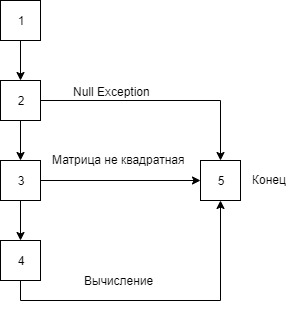
\includegraphics[width=.4\linewidth]{MatrixesExecutionFlowsGraph}}
        \hspace{.15\linewidth}
        \subfloat[Метод GetColumns]{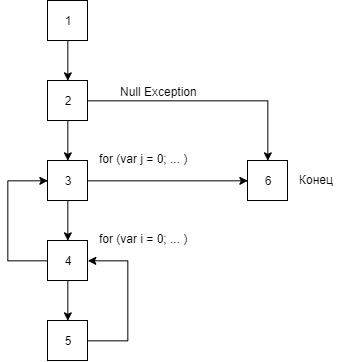
\includegraphics[width=.4\linewidth]{GetColumnsExecutionFlowsGraph}}
        \caption{Графы потоков управления первой программы}
    \end{figure}
    \pagebreak

    Вычислим цикломатическое число графа :
    \begin{equation*}
        C(G_{a}) = 6 - 5 + 2 = 3.
    \end{equation*}
    \begin{enumerate}
        \item 1, 2, 5.
        \item 1, 2, 3, 5.
        \item 1, 2, 3, 4, 5.
    \end{enumerate}

    Вычислим цикломатическое число графа:
    \begin{equation*}
        C(G_{b}) = 8 - 6 + 2 = 4.
    \end{equation*}
    \begin{enumerate}
        \item 1, 2, 6.
        \item 1, 2, 3, 6.
        \item 1, 2, 3, 4, 3, 6.
        \item 1, 2, 3, 4, 5, 4, 3, 6.
    \end{enumerate}

    \subsection{Тестирование программы № 2}
    Для программы работы над строками составим граф потоков управления.
    \begin{figure}[H]
        \centering
        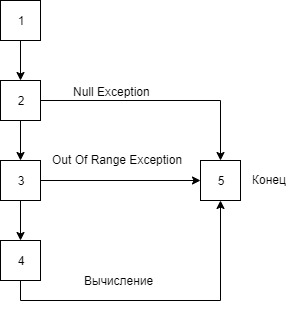
\includegraphics[width=.4\linewidth]{StringsExecutionFlowsGraph}
        \caption{Граф потоков управления второй программы}
    \end{figure}

    Вычислим цикломатическое число графа :
    \begin{equation*}
        C(G) = 6 - 5 + 2 = 3.
    \end{equation*}
    \begin{enumerate}
        \item 1, 2, 5.
        \item 1, 2, 3, 5.
        \item 1, 2, 3, 4, 5.
    \end{enumerate}

    \subsection{Тестирование программы № 3}
    Для программы работы над файлами составим граф потоков управления.
    \begin{figure}[H]
        \centering
        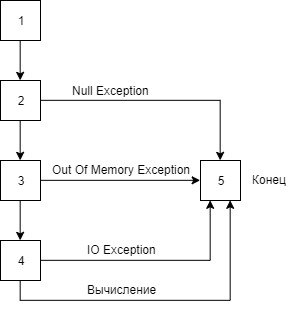
\includegraphics[width=.4\linewidth]{FileExecutionFlowsGraph}
        \caption{Граф потоков управления третьей программы}
    \end{figure}

    Вычислим цикломатическое число графа :
    \begin{equation*}
        C(G) = 7 - 5 + 2 = 4.
    \end{equation*}
    \begin{enumerate}
        \item 1, 2, 5.
        \item 1, 2, 3, 5.
        \item 1, 2, 3, 4, 5.
        \item 1, 2, 3, 4, 5.
    \end{enumerate}

    \section{Выводы}

    В ходе лабораторной работы было изучено структурное тестирование
    ПО (метод белого ящика) с использованием графа потоков управления.

    Преимуществом такого способа тестирования является уменьшение необходимой
    трудоемкости для тестирования программ. Обнаружились следующие недостатки:
    \begin{enumerate}
        \item Недостаточная глубина тестирования.
        \item Невозможность использования способа для крупных программ.
    \end{enumerate}

    Из-за слабого покрытия возможных вариантов входных данных, структурное 
    тестирование, по моему мнению, не является достаточным способом тестирования
    прогрммных модулей. Вместо него или, возможно, в дополнение к нему можно
    применить тестирование черным ящиком.

\end{document}